\section{系统测试}

测试是通过用例和预期结果检验系统行为的关键途径,
能够帮助开发人员快速检测出系统的问题。
在开发人员修改代码片段时,
测试能够快速提供开发人员关心的信息:
程序是否按预期执行?
如果与预期有偏差,具体是哪个行为不符合预期?
有问题的是哪个模块?
如果开发人员有了这些信息,
就能够知道系统是否待完善,
并能够快速定位问题根源,
从而提高软件开发的效率。

\subsection{测试用例的设计原则}

测试用例需要契合系统的接口,
对于本次研究的高层综合流程,
测试用例需要包含输入和输出代码。
输入代码直接作为流程的输入,
而输出代码需要有与预期一致的行为(代码不需要完全一样)。

为了使测试能够尽可能精确地反应系统特定部分的行为
(越精确意味着确定的范围越小),
测试的对象需要尽可能地小。
例如在系统输入相同的情况下,
有两个代码片段都有可能导致系统的同一个错误,
而这两个代码片段分别位于不同且可以分别测试的模块。
如果对整个系统进行该测试,
可能会使开发人员分辨不出来是哪个模块出了问题;
但如果将系统拆分为多个模块,
对这些模块单独测试,
开发人员便会更加轻松地定位到问题代码,
这样无疑是显著提高了测试的效率。

基于上述原则,
本次设计的高层综合流程采取了前端和后端分别测试的策略。
对于前端,测试输入是描述硬件的Python代码,
测试预期结果和输出是对应的XLS中间表示代码;
对于后端,测试输入是XLS中间表示代码,
输出则是行为相同的Verilog代码。

\subsection{前端测试}

为了能够完整地测试xlspy的各部分,
需要全面测试所有可能出现的语法,
并保证每个测试单元尽量只反应一种语法的行为。
与此同时,
测试集也需要一些较完整、贴近实际的代码,
既可以反应各模块之间的协同能力,
也可以确定系统能够处理常见规模的输入。

以赋值语句为例,
Python中的赋值语句支持在同一个语句对多个目标变量赋值,
那么编写测试用例时就可以在输入代码中包括多目标赋值,
并检测输出的中是否有多条右值相同,
目标不同的赋值语句,
并确保赋值的左右值一一对应。
针对编译器前端的测试用例清单如表\ref{table.2}所示。

\begin{table}[ht]
\begin{center}
\caption{测试用例表}

\begin{tabular}{ c c }
    \Xhline{3\arrayrulewidth}
    测试用例名             & 测试对象 \\
    \hline
    typed\_arg           & 带类型参数、运算符和返回值 \\
    mutable              & 常量、赋值语句以及变量 \\
    multiple\_op         & 赋值和各种运算符 \\
    complete\_branch     & 完整的分支语句、变量捕获 \\
    incomplete\_branch   & 不完整的分支语句、变量捕获 \\
    nested\_branch       & 嵌套分支语句 \\
    \Xhline{3\arrayrulewidth}
\end{tabular}

\label{table.2}
\end{center}
\end{table}

通过运行xlspy,
以测试用例Python代码文件作为输入,
可以生成对应的XLS中间表示。
以nested\_branch为例,
生成该用例的中间表示命令如图\ref{fig.5}所示。
通过输出重定向,
可以将中间表示存储到文件中。

\begin{figure}[h]
\centering 
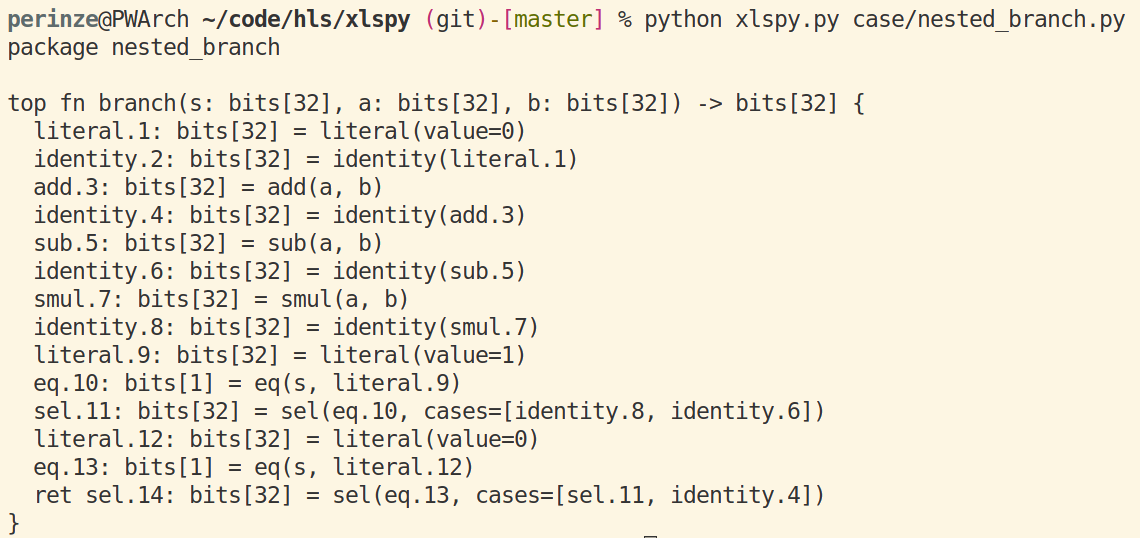
\includegraphics[width=0.9\textwidth]{figure/xlspy_command.png}
\caption{运行xlspy生成中间表示的命令}
\label{fig.5}
\end{figure}

XLS编译器提供了齐全的工具用于中间表示的操作,
本章用到的工具功能如表\ref{table.5}所示。
为了测试生成的中间表示行为是否符合预期,
需要借助XLS提供的eval\_ir\_main程序来运行中间表示,
同时用Python执行源代码,
判断对于一组相同的输入,
运行中间表示和运行Python源代码的结果是否一致,
从而判断中间表示是否与源代码具有相同的行为。
eval\_ir\_main运行中间表示的命令如\ref{fig.6}所示,
通过多组数据测试,
xlspy生成的中间表示行为均与Python源代码行为一致。

\begin{table}[ht]
\begin{center}
\caption{XLS工具功能表}

\begin{tabular}{ c c }
    \Xhline{3\arrayrulewidth}
    工具名称              & 功能 \\
    \hline
    eval\_ir\_main       & 根据用户提供的输入对中间表示求值并返回结果 \\
    opt\_main            & 对中间表示进行分析、代码变换和优化 \\
    ir\_viz              & 中间表示可视化分析工具,可以分析数据流 \\
    codegen\_main        & 从中间表示生成Verilog代码 \\
    \Xhline{3\arrayrulewidth}
\end{tabular}

\label{table.5}
\end{center}
\end{table}

\begin{figure}[h]
\centering
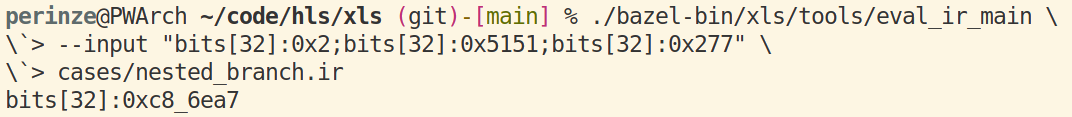
\includegraphics[width=0.9\textwidth]{figure/eval_ir_command.png}
\caption{中间表示的执行}
\label{fig.6}
\end{figure}

\subsection{后端测试}

%由于本次设计的高层综合流程是基于XLS工具设计的,
%在设计测试时,并不需要为依赖的且没有被修改的部分添加测试。
%具体而言,
%因为我并没有修改codegen部分的代码,
%所以并不需要另外编写codegen的测试;
%opt除了ir\_parser以及pass中除了TypeExpansionPass,
%其它部分也没有测试的必要。

%在第\ref{ir_parser}节我们介绍了对ir\_parser的扩展,
%为其添加了动态类型的解析规则,
%所以这部分的测试需要检查带有动态类型的是否被解析为一个类型列表,
%且列表里的所有类型与一致。
%测试TypeExpansionPass时,
%则需要检查输入的动态类型是否被展开为多个对应类型的模块,
%并且有对应的多路复用器根据类型信号选择对应的计算结果。

后端可以拆分为两个部分,
分别是中间表示优化和代码生成。
本节将分别介绍对这两部分的功能测试,
中间表示优化部分测试对中间表示的优化能力,
而代码生成部分测试生成代码与源代码是否等效。

\subsubsection{中间表示优化器测试}

XLS的优化效果可以通过各测试用例优化前后的中间表示代码行数来展现,
这样做的依据在于XLS中间表示每行仅有一个操作符,
对应到硬件即为一个运算单元,
中间表示代码行数的减少能够大致反应硬件面积的减少。
运行opt\_main对中间表示进行优化的命令如图\ref{fig.7}所示,
图中分别为优化前后的中间表示,
可以看到优化后中间表示代码行数明显减少。

\begin{figure}[h]
\centering
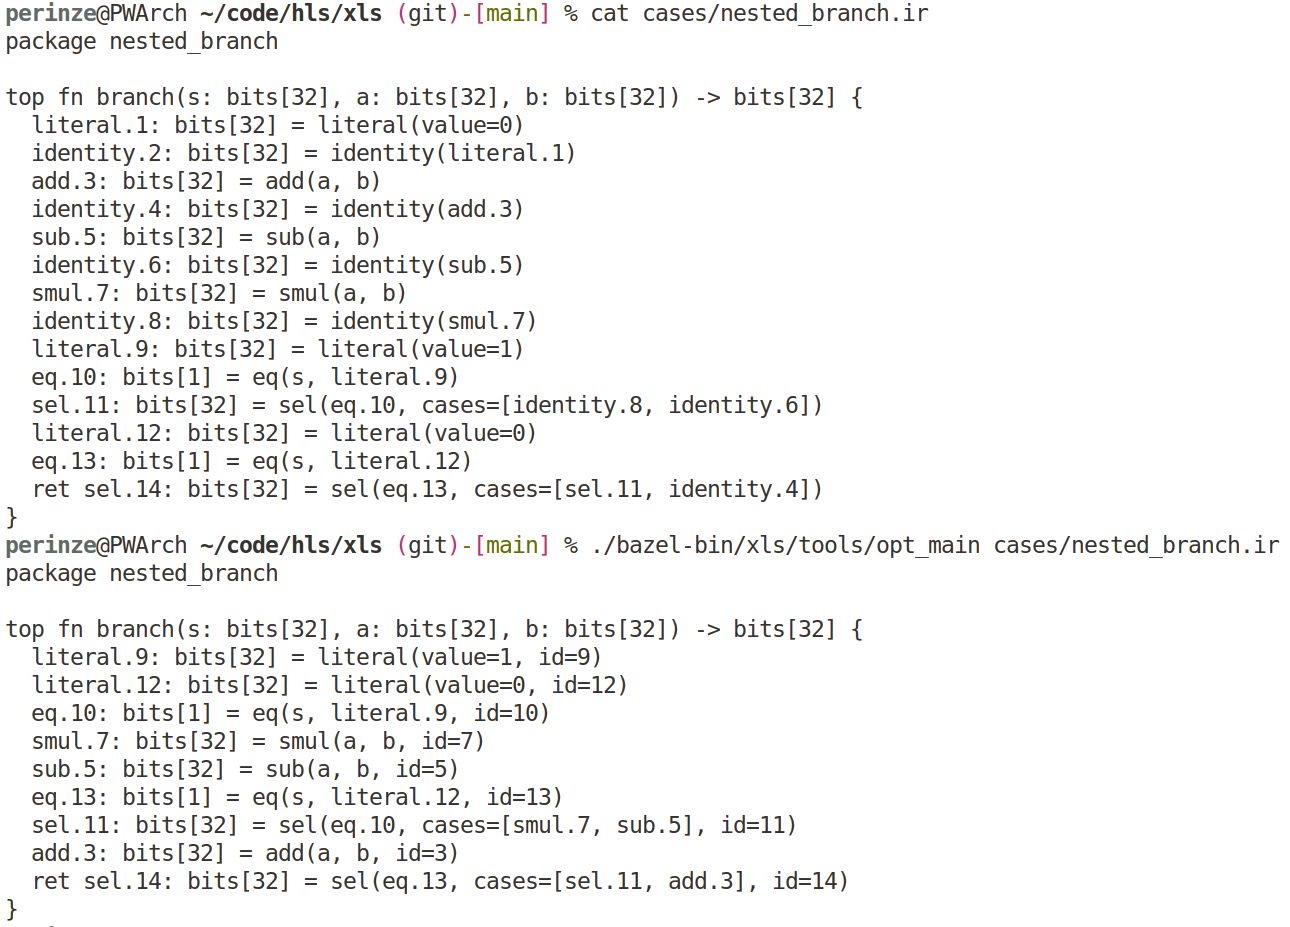
\includegraphics[width=0.9\textwidth]{figure/opt_command.png}
\caption{nested\_branch.ir优化前后对比}
\label{fig.7}
\end{figure}

对所有测试用例的中间表示进行优化,
各测试用例优化前后函数体代码行数对比表格如\ref{table.7}所示。
去掉mutable等欠缺代表性的用例,
其余用例的平均优化能力大约为0.6x,
可以大致反映优化器对大多数代码的优化能力。

\begin{table}[ht]
\begin{center}
\caption{各用例优化前后代码行数对比表}

\begin{tabular}{ c c c }
    \Xhline{3\arrayrulewidth}
    测试用例名             & 优化前行数 & 优化后行数\\
    \hline
    typed\_arg            & 1  & 1 \\
    single\_op            & 1  & 1 \\
    mutable               & 7  & 1 \\
    multiple\_op          & 7  & 4 \\
    complete\_branch      & 9  & 5 \\
    incomplete\_branch    & 9  & 6 \\
    nested\_branch        & 14 & 9 \\
    \Xhline{3\arrayrulewidth}
\end{tabular}

\label{table.7}
\end{center}
\end{table}

XLS也提供了一个中间表示可视化工具,
可以用于分析代码结构是否正确,
以及计算过程中可能的数据流向。
例如在nested\_branch这一例子中,
当s不等于0或1时,
数据流向如图\ref{fig.8}左半部分;
而s等于0时,
数据流向如图\ref{fig.8}右半部分。
这也体现了在该测试用例中,
s值的不同影响着代码的数据流向。

\begin{figure}[h]
\centering
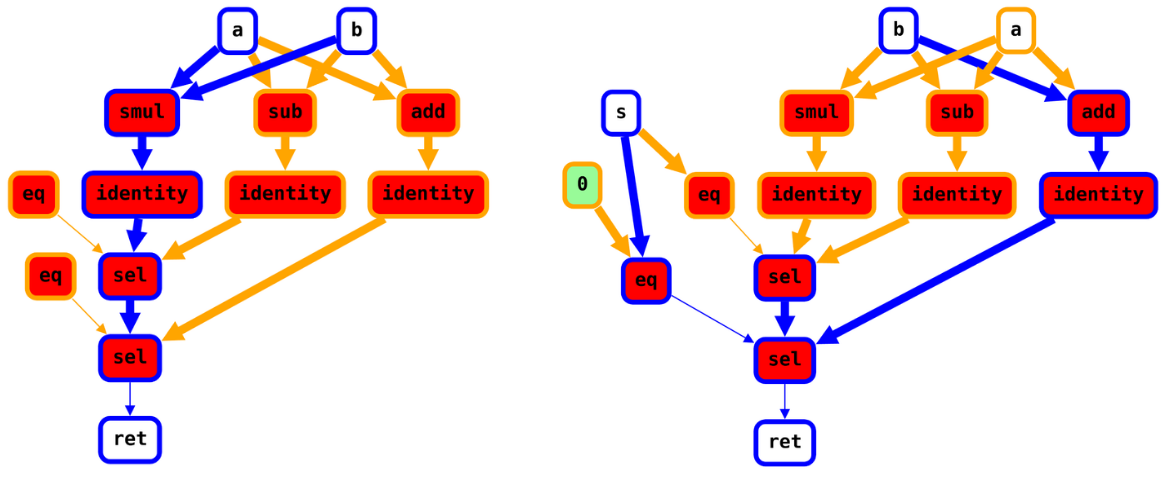
\includegraphics[width=0.85\textwidth]{figure/ir_viz.png}
\caption{nested\_branch的两种数据流图}
\label{fig.8}
\end{figure}

\pagebreak

\subsubsection{代码生成测试}

Verilog代码生成是整个流程的最终目的,
我们需要测试生成的Verilog是否符合我们的期望。
XLS的代码生成器命令示例如图\ref{fig.11}所示,
命令中分别指定了生成器类型(这里为组合逻辑生成器)、
时延模型、输出Verilog代码路径和模块名,
以及输入的中间表示代码的顶层函数名和文件名,
而图\ref{fig.11}的下半部分展示了生成的Verilog代码,
其行为与源代码、中间表示代码均一致。
由于流程中默认采用有符号整数乘法,
在Verilog中表示有符号乘法涉及到一些类型转换,
所以XLS生成的Verilog代码中出现了一个函数,
用于包装有符号乘法需要的所有操作。

\begin{figure}[h]
\centering
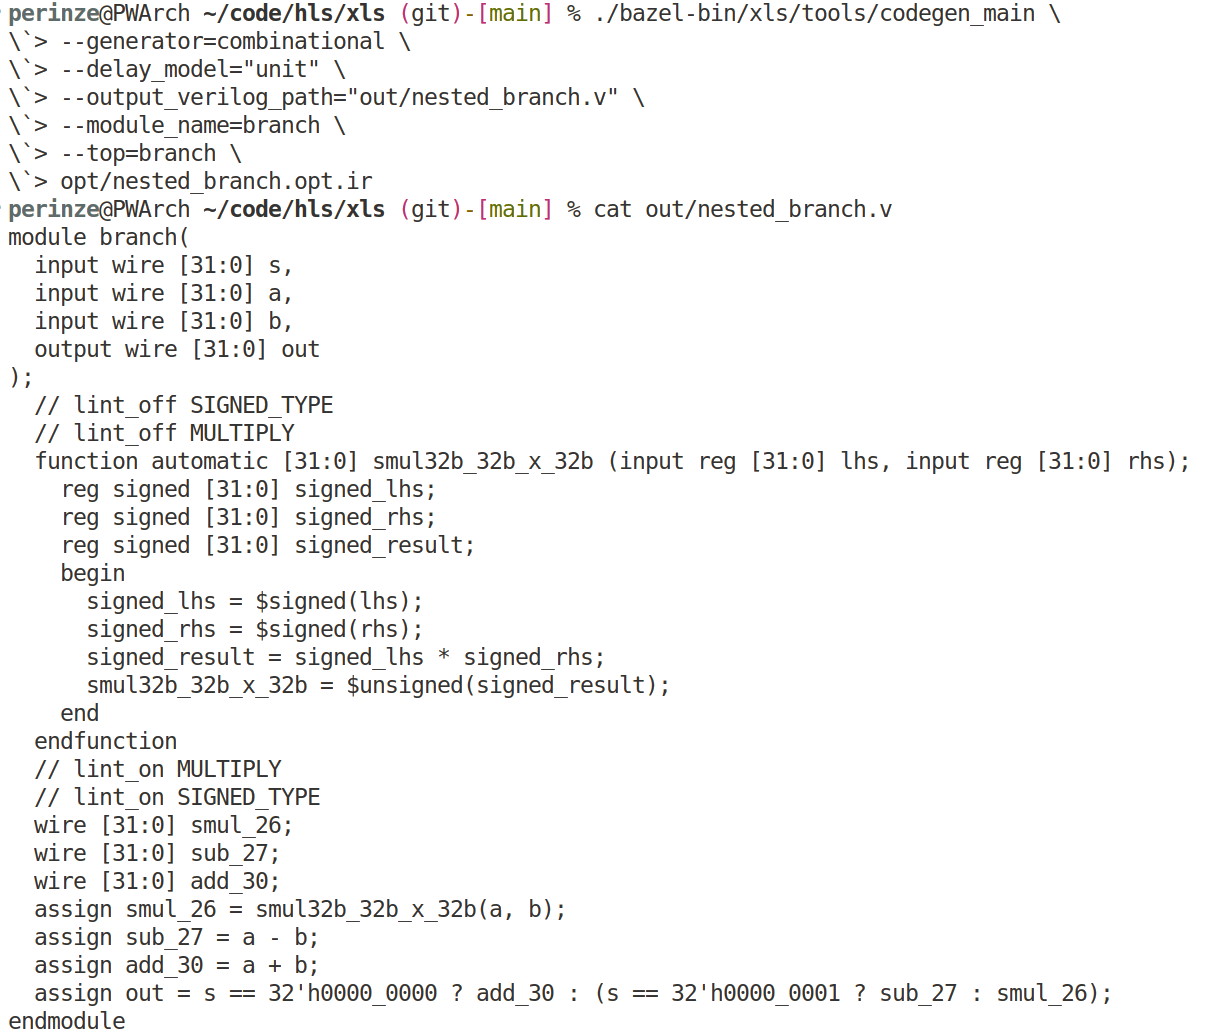
\includegraphics[width=0.9\textwidth]{figure/codegen_command.png}
\caption{代码生成器命令及输出代码}
\label{fig.11}
\end{figure}

对于生成的Verilog代码,
本文通过Icarus Verilog仿真工具测试其行为。
以nested\_branch为例,
为待测试的Verilog模块编写testbench并仿真,
结果如\ref{fig.12}和\ref{fig.13}所示。
图中结果的输入输出数据均与\ref{fig.6}一致,
其它数据经测试也与前端测试行为一致。

\begin{figure}[h]
\centering
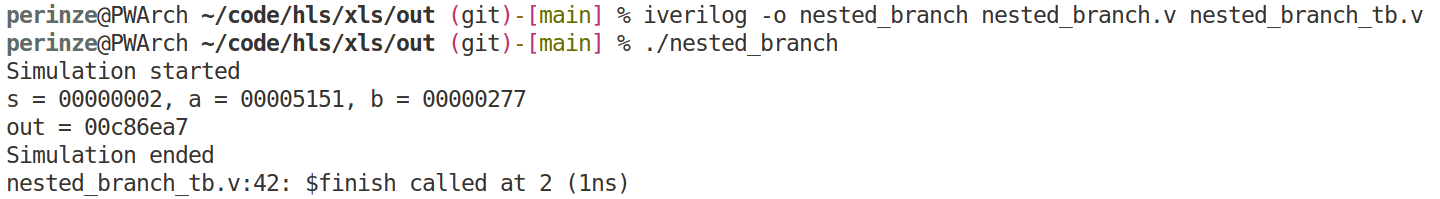
\includegraphics[width=0.9\textwidth]{figure/verilog_test.png}
\caption{Verilog代码测试}
\label{fig.12}
\end{figure}

\begin{figure}[h]
\centering
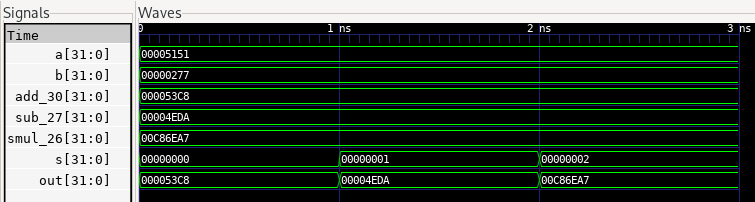
\includegraphics{figure/wave.png}
\caption{Verilog代码测试波形图}
\label{fig.13}
\end{figure}

\pagebreak

\subsection{浮点数运算单元测试}

在系统设计中我们以XLS中间表示的形式设计了浮点运算单元。
为了测试浮点运算单元正确性,
需要编写脚本生成所有浮点数组合并保存到输入文件中
通过Icarus Verilog的输入输出功能,
将输入数据连同浮点运算单元的输出保存到结果文件中,
再运行验证脚本检查结果文件数据是否与C语言浮点数运算结果一致。
经过验证,所有浮点数运算结果无误,
浮点数运算单元行为正确。

\subsection{本章小结}

本章完成了对本设计的高层综合流程前端代码生成、
后端代码优化和生成以及浮点数运算正确性测试,
并通过对比优化前后代码量展示了优化能力,
同时也对生成的Verilog代码进行仿真验证,
验证了本设计的有效性。